\documentclass[crop,tikz]{standalone}%
\usepackage[margin=1in]{geometry}
\usepackage{libertine}
\usepackage{amssymb}
\usepackage{ulem}
\usepackage{../macro}

\newcommand{\xbar}[1]{\ensuremath{\overline{\textrm{#1}}}}

\usepackage[table,dvipsnames]{xcolor}
\usepackage{graphicx}
\usetikzlibrary{positioning}% To get more advances positioning options

\begin{document}

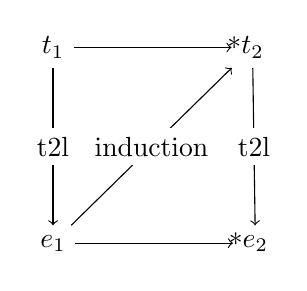
\begin{tikzpicture}[]
    \node (t1) at (0,0) {$t_1$};
    \node (t2) [right=2cm of t1]  {$t_2$};
    \node (e1) [below=2cm of t1]  {$e_1$};
    \node (e2) [right=2cm of e1]  {$e_2$};
    % letf to right arrows
    \draw [->] (t1) -- (t2)node[pos=1,xshift=1pt]{*}; ;
    \draw [->] (e1) -- (e2)node[pos=1,xshift=1pt]{*};

    % up to down arrows
    \path [->] (t1) edge node[fill=white, anchor=center]{t2l} (e1);
    \path [->] (t2) edge node[fill=white, anchor=center]{t2l} (e2);

    % diagonal arrow
    \path[->] (e1) edge node[fill=white, anchor=center, pos=0.5] {induction} (t2);
\end{tikzpicture}


\end{document}
